\documentclass[10pt,twocolumn,letterpaper]{article}

\usepackage{cvpr}
\usepackage{float}
\usepackage{times}
\usepackage{epsfig}
\usepackage{graphicx}
\usepackage{amsmath}
\usepackage{amssymb}
\usepackage{caption}
\usepackage{multirow}

\newcommand\fnote[1]{\captionsetup{font=small}\caption*{#1}}


% Include other packages here, before hyperref.

% If you comment hyperref and then uncomment it, you should delete
% egpaper.aux before re-running latex.  (Or just hit 'q' on the first latex
% run, let it finish, and you should be clear).
\usepackage[breaklinks=true,bookmarks=false]{hyperref}

\cvprfinalcopy % *** Uncomment this line for the final submission

\def\cvprPaperID{****} % *** Enter the CVPR Paper ID here
\def\httilde{\mbox{\tt\raisebox{-.5ex}{\symbol{126}}}}

% Pages are numbered in submission mode, and unnumbered in camera-ready
%\ifcvprfinal\pagestyle{empty}\fi
\setcounter{page}{1}
\begin{document}

%%%%%%%%% TITLE
\title{Classification on the Google's Quickdraw Dataset}

\author{Rémi Calixte\\
CentraleSupélec\\
{\tt\small remi.calixte@student.ecp.f}
% For a paper whose authors are all at the same institution,
% omit the following lines up until the closing ``}''.
% Additional authors and addresses can be added with ``\and'',
% just like the second author.
% To save space, use either the email address or home page, not both
\and
Corentin Dupret\\
CentraleSupélec\\
{\tt\small corentin.dupret@student.ecp.fr}
\and
Sami Tabet\\
CentraleSupélec\\
{\tt\small sami.tabet@student.ecp.fr}
}

% Variables
\newcommand{\rnnTitle}{Recurrent Neural Networks on the drawn strokes}
\newcommand{\cnnTitle}{Convolutional Neural Networks on 28x28 grayscale bitmaps}
\newcommand{\imgenTitle}{Transfer Learning of Convolutional Neural Networks on 64x64 and 96x96 images generated from drawn strokes}


\maketitle
%\thispagestyle{empty}

%%%%%%%%% ABSTRACT
% \begin{abstract}    
%    The ABSTRACT is to be in fully-justified italicized text, at the top
%    of the left-hand column, below the author and affiliation
%    information. Use the word ``Abstract'' as the title, in 12-point
%    Leave two blank lines after the Abstract, then begin the main text.
%    Look at previous CVPR abstracts to get a feel for style and length.
% \end{abstract}

%%%%%%%%% BODY TEXT
\section{Introduction}

In this study we focus on the classification of drawings realized by participants of the game Quickdraw \cite{GoogleQuickdraw}. Quickdraw is a game released by Google that prompts the participant with the name of an item  (for instance drums), the participant then has 20 seconds to draw it and make a neural network guess the correct item name. Thanks to this game, the Quickdraw team collected a lot of annotated images and made them available publicly, there are 345 different items and each has at least $100,000$ samples.

We study different classifiers using different forms of data that range from strokes data to images. All the code used in this study can be found \href{https://github.com/cs-deep-quickdraw/notebooks}{here: https://github.com/cs-deep-quickdraw/notebooks}.

Our goal is to get the best possible accuracy on 100 different classes of drawings.

%-------------------------------------------------------------------------


%------------------------------------------------------------------------
\section{Prior Work}

Many different projects arose from the Quickdraw dataset \cite{GoogleQuickdraw}. Some are data analyses, others are artistic projects, often based on image generation. However, we are especially interested in projects that use this dataset for classification as this is the problem we want to solve in this study.

Fortunately, Google Research created a competition on Kaggle for classifying drawings from this dataset \cite{KaggleCompetition}. The data is available as strokes from the drawings. Most of the solutions for this competition use two different approaches: a LSTM trained on the strokes \cite{KaggleLSTM} or a CNN trained on images generated from the strokes \cite{KaggleCNN} \cite{KaggleMobileNet}. Big models such as ResNet34 \cite{KaggleResNet} and MobileNet \cite{KaggleMobileNet} perform well on this classification task. The best solutions use ensemble methods with their best models \cite{KaggleFirstPlace} (and even snapshot ensemble methods to have more models in the ensemble \cite{KaggleFifthPlace}). The authors of the first place solution give a list of good CNN architectures to try for this problem: "resnet18, resnet34, resnet50, resnet101, resnet152, resnext50, resnext101, densenet121, densenet201, vgg11, pnasnet, incresnet, polynet, nasnetmobile, senet154, seresnet50, seresnext50, seresnext101". \cite{KaggleFirstPlace}

It should be noted that the dataset we are using also provides data in another format than the one used in the competition so we can even try other approaches.

%------------------------------------------------------------------------
\section{Approaches}

In this section we detail, from a theoretical perspective, the three approaches that we investigate to obtain the best possible performance on our classification task.

%------------------------------------------------------------------------
\subsection{\rnnTitle{}}

The first approach we investigate is based on the usage of the processed drawn strokes \cite{GoogleQuickdraw}.

As it's name implies, it's a processed version of the raw dataset to make it easier to use by doing the following transformations on the raw dataset \cite{GoogleQuickdraw}:

\begin{itemize}
    \item Aligning the drawings to the top-left corner, to have minimum values of 0.
    \item Uniformly scaling the drawings, to have a maximum value of 255.
    \item Resampling all strokes with a 1 pixel spacing.
    % https://en.wikipedia.org/wiki/Ramer%E2%80%93Douglas%E2%80%93Peucker_algorithm
    \item Simplifying all strokes using the Ramer–Douglas–Peucker \cite{wiki:rdp_algo} algorithm with an epsilon value of 2.0.
\end{itemize}

The first two transformations are to account for the different devices the participants played on that had different sizes, the two others are here to "reduce" the complexity of the drawings.

Since the preprocessed dataset is already "normalized" it makes more sense for us to use this one rather than the raw one. Moreover, the fact that strokes already had been simplified makes it lighter memory-wise than the raw one making it faster to load and to train on.


\begin{figure}[h] 
\centering
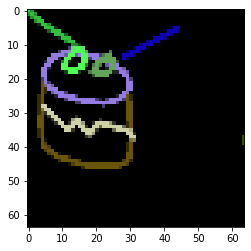
\includegraphics[width=0.15\textwidth]{images/drums_quickdraw_strokes_202.png}
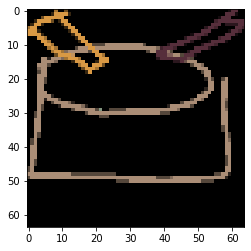
\includegraphics[width=0.15\textwidth]{images/drums_quickdraw_strokes_25001.png}
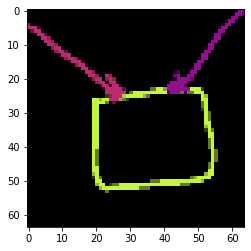
\includegraphics[width=0.15\textwidth]{images/drums_quickdraw_strokes_25019.png}
\caption{Samples of the quickdraw's dataset \textit{drums} class, each color represent a different stroke}
\label{fig:drums_strokes}
\end{figure}

This dataset is available in \texttt{.bin} format (raw bytes) and \texttt{.ndjson}, for performance purposes we will use the \texttt{.bin} format.

A number of fields are available per image (\texttt{key\_id}, \texttt{country\_code}, \texttt{timestamp}) however we will solely focus on the strokes. In this dataset a stroke is represented by a list of ($x$, $y$) coordinates on the canvas. Whenever the participant lifts the pencil, the stroke ends.

So for each image, we have an associated list of strokes. To encode the information of "lifting the pencil" we decide to use the same solution as in the Tensorflow's RNNs tutorial \cite{TensorflowTutorial}: adding a third value to the coordinates to indicate if the current point is the end of a stroke or not. Hence the list of list of ($x$, $y$) coordinates becomes a simple list of ($x$, $y$, $last$) tuples where $last \in \{0, 1\}$ indicates whether or not the current point is the end of a stroke. We also normalize the coordinates within each image to have values in $[0, 1]$ for $x$ and $y$.

To exploit the fact that these strokes are sequential data, we decide to use Recurrent Neural Networks (RNNs) because they are very well suited for temporal/sequential data. More precisely, we will use Long short-term memory neural networks \cite{DBLP:journals/corr/GreffSKSS15} that are a specific type of RNNs which architectures are described on figure \ref{fig:lstm}. This architecture has the benefits of solving the vanishing gradient issue that sometimes raises when using RNNs and mitigates the exploding gradient problem without tackling it completely.



\begin{figure}[h] 
\centering
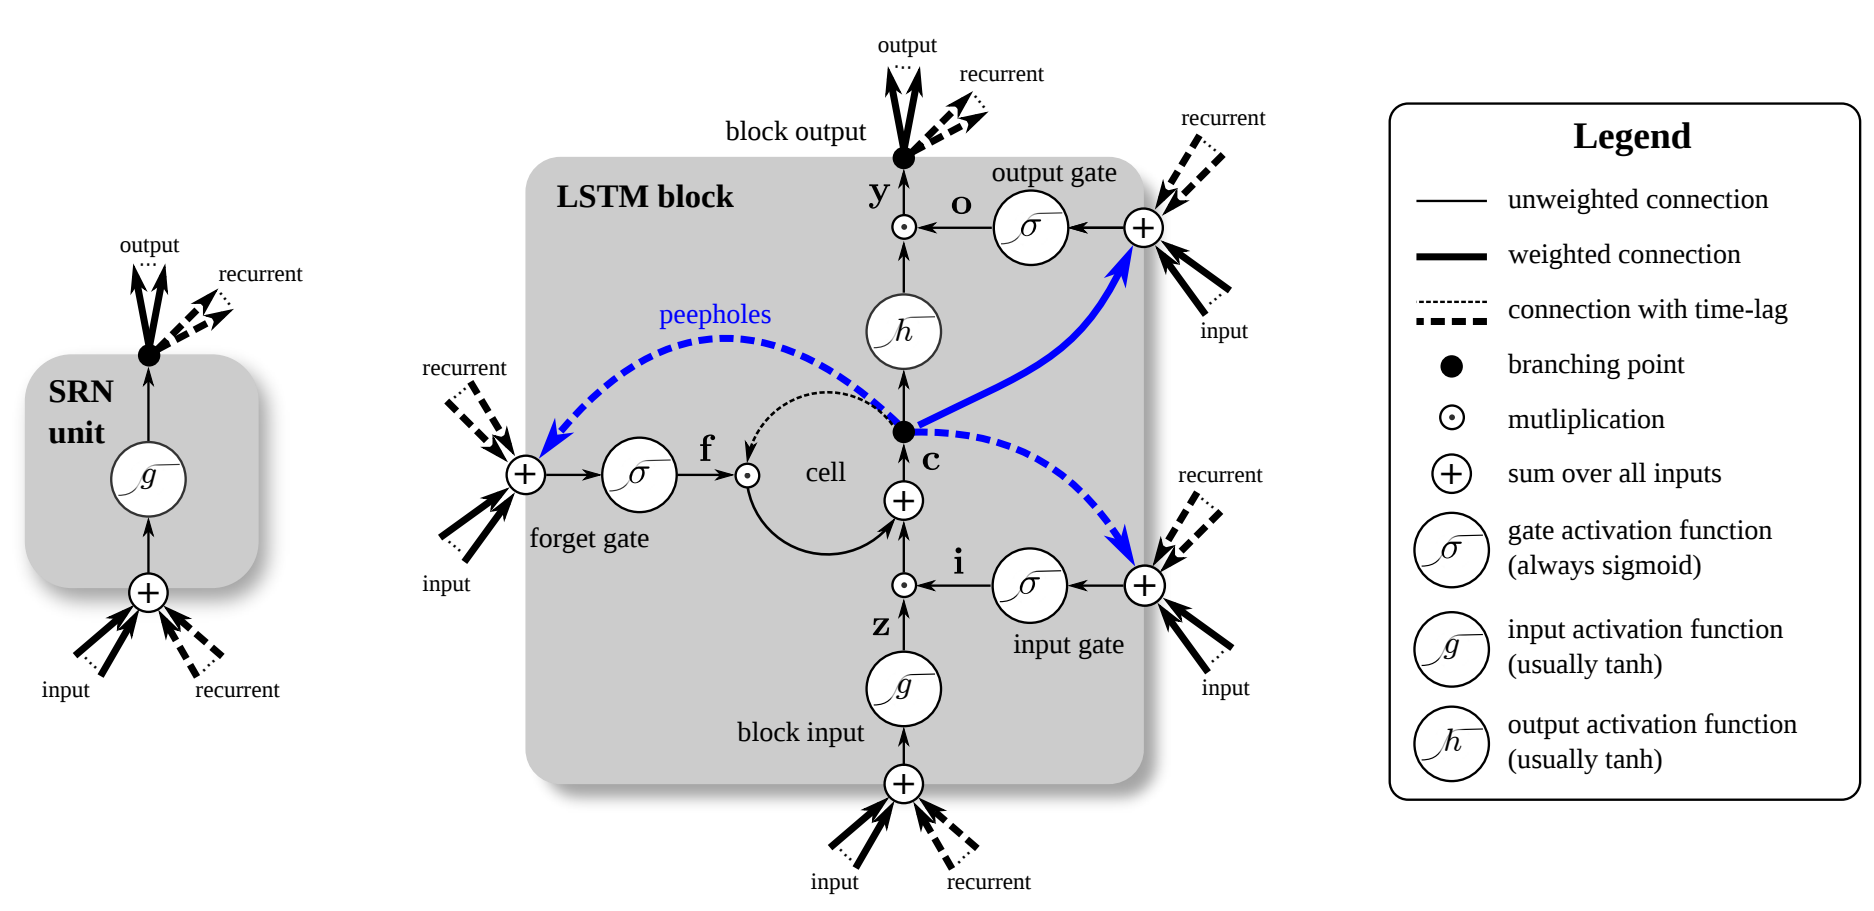
\includegraphics[width=0.45\textwidth]{images/lstm.png}
\caption{Detailed schematic of the Simple Recurrent Network (SRN) unit (left) and a Long Short-Term Memory block (right) as used in the hidden layers of
a recurrent neural network. \cite[p.~2]{DBLP:journals/corr/GreffSKSS15}}
\label{fig:lstm}
\end{figure}

We also try to add 1 dimension convolutions layers before the LSTM to see if these can extract meaningful features from the raw coordinates.

%------------------------------------------------------------------------
\subsection{\cnnTitle{}}

The second approach we investigate is based on the usage of another format for the preprocessed dataset. The simplified drawings have been rendered into 28x28 grayscale bitmaps in numpy (\texttt{.npy}) format. Not only is this format easy to use in practice (files are easily loaded in memory by using \texttt{numpy}), but it is also memory-efficient as the 1-channel images are very small. Some samples of the bitmap dataset are shown in figure \ref{fig:bitmap_drums}.

\begin{figure}[h] 
\centering
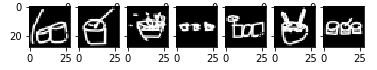
\includegraphics[width=0.45\textwidth]{images/bitmaps_drums.png}
\caption{Samples of the \textit{drums} class from the quickdraw bitmap dataset}
\label{fig:bitmap_drums}
\end{figure}

To exploit this dataset, we decide to use Convolutional Neural Networks (CNNs) because they are remarkably suited for processing data that is intrinsically organized as a grid, such as images. This makes CNNs the most popular neural network model being used for image classification problem, so trying to use them for our problem was mandatory.

A CNN is a neural network with at least one convolution layer, \textit{i.e.} a layer where convolution is used instead of matrix multiplication. Generally, CNNs contain several convolution layers (to generate "feature maps") followed by fully connected layers (which typically use these feature maps for classification). An example of CNN is shown in figure \ref{fig:lenet5}.

\begin{figure}[h] 
\centering
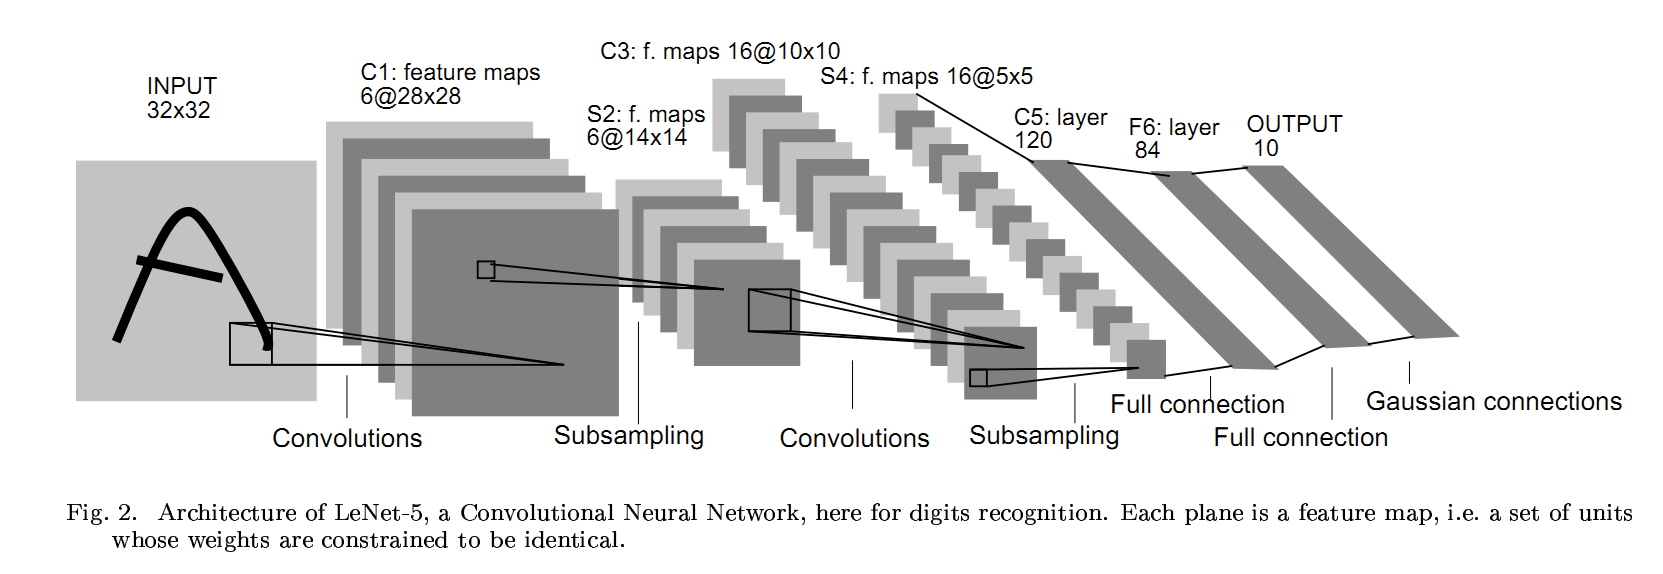
\includegraphics[width=0.45\textwidth]{images/cnn_lenet5.png}
\caption{Architecture of LeNet-5, a CNN used here for digits recognition. \cite{lecun-98}}
\label{fig:lenet5}
\end{figure}

In this approach, we try different tried and proven image classification CNN models that happen to also be suitable for processing 28x28 images, namely ResNet18, ResNet34, and MobileNet.

ResNet is a special kind of CNN architecture introduced in 2015 \cite{he2016deep} that addresses the problem of vanishing gradients by using "skip connections" that connect one layer to another while jumping over some layers in between.

MobileNet is a CNN architecture introduced in 2017 \cite{howard2017mobilenets} in order to improve the efficiency of convolutions for mobile vision applications, while keeping great performances. It uses "depthwise separable convolution", a special kind of convolution in two steps:

\begin{itemize}
    \item a depthwise convolution, where kernels are applied to a single channel (as opposed to classical convolution where kernels are applied simultaneously to all channels)
    \item a pointwise convolution, where 1x1x3 kernels are applied to the output of the depthwise convolution to combine them into feature maps.
\end{itemize}

This kind of convolution uses much less operations than the classical convolution.

%------------------------------------------------------------------------
\subsection{\imgenTitle{}}

The last approach we try is based on the observation that 28x28 is a rather small format for the type of drawings we study. We thus render the same simplified drawings in grayscale ourselves with \texttt{numpy} and \texttt{opencv} to work with greater resolutions.

Within a given memory envelope, increasing the size of the images is at the expense of the number of images we can store and on which we can learn. This is why we choose the still rather moderate resolutions of 64x64 and 96x96.

This newly generated dataset is used on the same models than for the 28x28 dataset since the structure of the data is the same. However we experiment with the pretrained version of these models to hopefully speed up the learning and get better results.

%------------------------------------------------------------------------
\section{Experiments}

In this section, we detail, comment, and interpret the results obtained for each one of the three approaches.

%------------------------------------------------------------------------
\subsection{Experimental protocols and performance measures}

All the approaches are using the same test images: the first $20,000$ samples of each class. This is to be able to compare correctly the results that each approach yields. Moreover, the loss function used by each approach is also the same: the cross entropy loss, so the validation losses could also be compared, however since we are not using the same training strategies for each approach (batch size, learning rate, optimizer, samples of training) we won't do any comparison on this.

%------------------------------------------------------------------------
\subsection{\rnnTitle{}}

In this subsection, the word \texttt{image} will refer to a list of augmented coordinates $(x, y, last)$ as described earlier.

The models trained for this approach range from the simple one layer LSTM to more complex models comporting convolutions layers and multi layers BiLSTM.

First, to be able to batch multiple \texttt{images} they need to have the same sequence length within a batch. To achieve that, we do a preliminary study of the count of coordinates distribution among the dataset:

\begin{table}[h]
    \centering
    \begin{tabular}{c|c|c|c|c}
          & \textbf{Mean} & \textbf{p90} & \textbf{p95} & \textbf{p99} \\
          \hline
         values & 43 & 77 & 96 & 137
    \end{tabular}
    \caption{Statistical distribution of the count of augmented coordinates per \texttt{image} among the quickdraw dataset}
    \label{tab:strokes_stats}
\end{table}

Hence we choose to normalize the sequence length of each \texttt{image} to $100$. In practice, this is done by adding $(0, 0, 0)$ elements to the \texttt{images} with less than $100$ coordinates, and keeping only the first $100$ coordinates for the \texttt{images} with more than $100$ coordinates.

Another interesting approach would be to have a smaller window (for instance $75$) that would be a sliding window. Hence, if an \texttt{image} has $125$ coordinates, we could split it into multiple \texttt{images} made of a subset of the initial strokes, for instance: coordinates $0$ to $75$, coordinates $10$ to $85$, etc. 
In this study we go with the simpler padding or cropping approach rather than the sliding window one.

The effect of increasing the length of the sequence is a compromise between having more meaningful data for \texttt{images} with long sequence lengths and adding a lot of noise to \texttt{images} with smaller sequence lengths. 


The models were trained on $20,000$ \texttt{images} per class (hence $2,000,000$ in total) and with a validation set of $4,000$ \texttt{images} per class (hence $400,000$ in total).

All the models in this section were trained using the \texttt{Adam} optimizer \cite{kingma2014adam} with a learning rate of $10e^{-3}$ and with batches containing 256 \texttt{images}. Moreover, they all used a layer of batch normalization \cite{ioffe2015batch} at the entry of the neural network for regularization purposes. 


\subsubsection{LSTMs networks without convolutions}

In this section we present the results obtained for LSTMs networks without convolutions layers.

The trained models were 1 layer LSTMs with hidden layer sizes of 64 and 256 and 2 layers LSTMs with hidden layers sizes of 64, 128 and 256. The results are available on figure \ref{fig:lstm_results}.

\begin{figure}[h] 
\centering
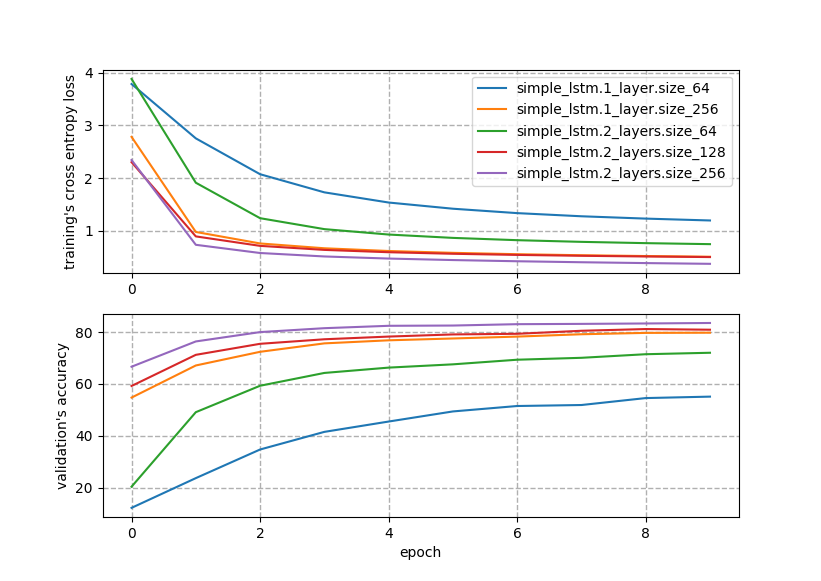
\includegraphics[width=0.45\textwidth]{images/simple_lstm_results.png}
\caption{Results for LSTMs networks without convolutions layers}
\label{fig:lstm_results}
\end{figure}

The first thing we can notice is that adding one more LSTM layer is less impactful than increasing the size of the LSTM hidden layer, the 1 layer LSTM with a hidden size of 256 performed better on the validation set than the 2 layers LSTM with hidden sizes of 64. However this is less and less pronounced as we increase the size of the hidden sizes as we can see with the 2 layers LSTM with a hidden sizes of 128 (maximum validation accuracy of $81.15\%$) and the one with hidden sizes of 256 (maximum validation accuracy of $83.49\%$). Finally, we notice that the bigger models are plateauing quickly (both for the validation accuracy and the training loss), which could mean that we could probably have better results with more complex models.

Training similar models with BiLSTMs (Bidirectional LSTM) instead of LSTMs yields similar results and does not improve significantly the results described in figure \ref{fig:lstm_results} we have very similar results. The BiLSTM results are shown on figure \ref{fig:bilstm_results}, the best validation accuracy is reached by a 2 layers BiLSTM with hidden sizes of 256 and is $83.51\%$.

\begin{figure}[h] 
\centering
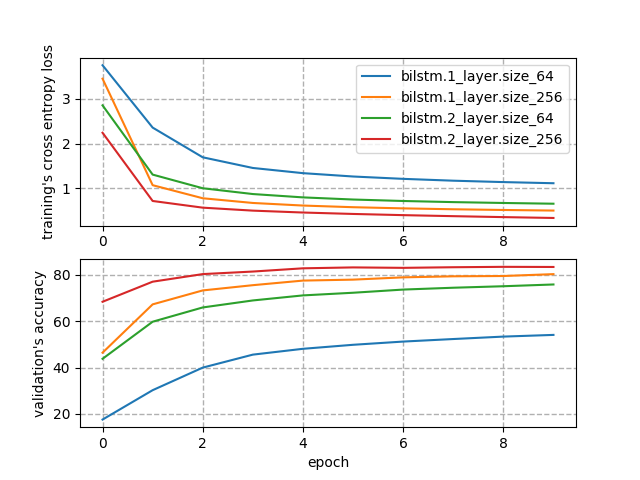
\includegraphics[width=0.45\textwidth]{images/simple_bilstm_results.png}
\caption{Results for BiLSTMs networks without convolutions layers}
\label{fig:bilstm_results}
\end{figure}


\subsubsection{LSTMs networks with convolutions}

In this section we present the results obtained for LSTMs networks with convolutions layers.

The convolutions layers are added before the LSTMs and just after the batch normalization layer \cite{ioffe2015batch}, the \texttt{channels} used for the input data are the $x$ coordinate, the $y$ coordinate and the $last$ flag.

The goal of these convolutions layers is to extract more meaningful data from the coordinates before forwarding it to the LSTM part of the network, these architectures are highly inspired by the Tensorflow's sketch RNN \cite{TensorflowTutorial}.

\begin{figure}[h] 
\centering
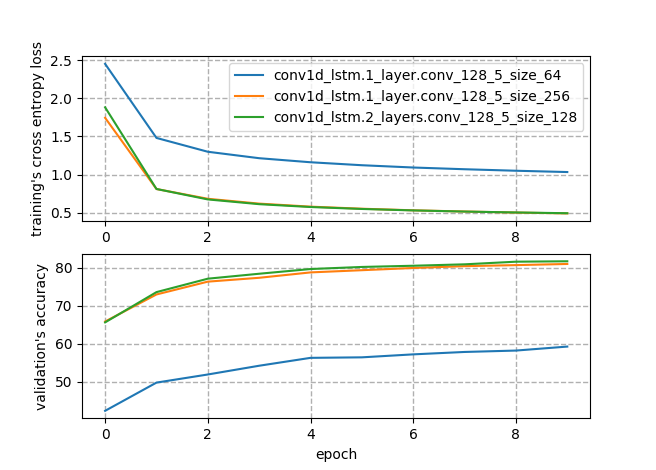
\includegraphics[width=0.45\textwidth]{images/conv_lstm_results.png}
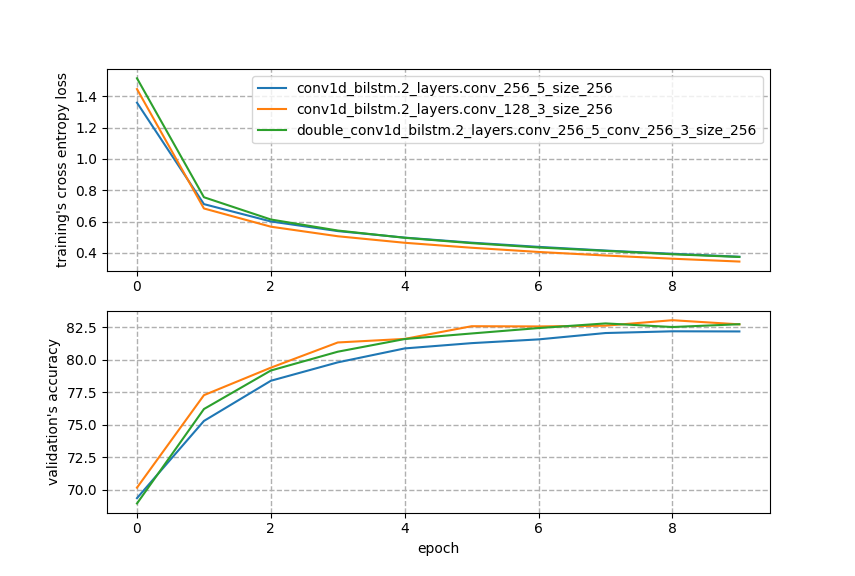
\includegraphics[width=0.45\textwidth]{images/conv_bilstm_results.png}
\caption{Results for LSTMs/BiLSTM networks with convolutions layers}
\label{fig:conv_lstm_results}
\end{figure}

The first thing we notice on the results of figure \ref{fig:conv_lstm_results} is that as opposed to the NN without convolutions layers, the one with convolutions layers are better if the LSTM part is bidirectional. This might be explained by the fact that the input data of the LSTMs with convolutions are more complex (they have a bigger dimension), hence the LSTM being bidirectional can detect more "patterns" in the data.

The second thing is that having two layers of convolutions does not significantly increase the performance of the model compared to having just one. This might be explained by the fact that the convolution layers are already much more bigger than the input data making it harder to stack them while keeping "interesting" feature maps.

We can also see that having a convolution layer before a small LSTM (hidden size of 64) did not affect the performance of the model (compared to the results presented in figure \ref{fig:lstm_results}). This might be explained by the fact that the LSTM without a convolution layer already had trouble learning patterns and this did not improve when giving it bigger input data.

We finally choose to train a BiLSTM with 2 convolutions layers on the whole dataset ($75,000$ \texttt{images} per class for training and $15,000$ for validation). The first takes $3$ input channels and outputs $256$ channels with a kernel size of $5$, the second takes $256$ input channels and outputs $256$ channels with a kernel size of $3$, then this is forwarded to a 2 layers BiLSTM of hidden layer sizes of 256. The results are shown on figure \ref{fig:final_lstm_results}.

\begin{figure}[h] 
\centering
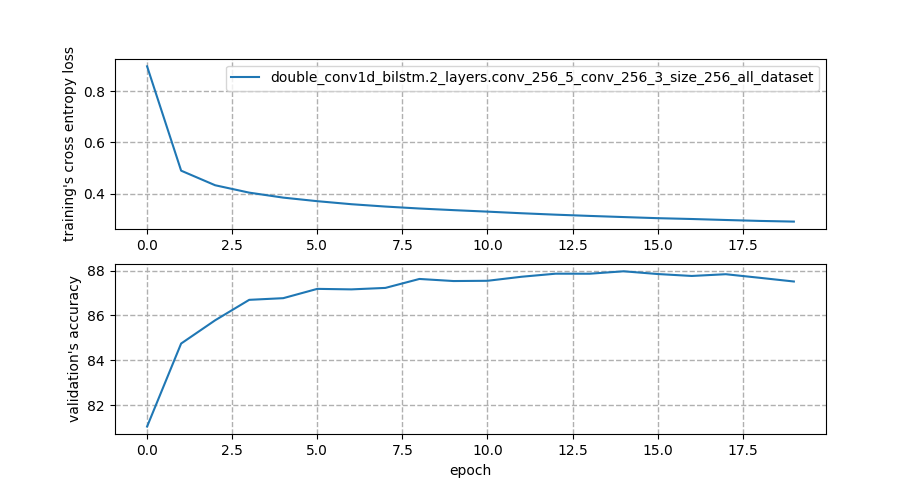
\includegraphics[width=0.45\textwidth]{images/lstm_final_result.png}
\caption{Results for the final BiLSTM network chosen}
\label{fig:final_lstm_results}
\end{figure}

We notice a big improvement ($+5.5\%$ of validation accuracy) compared to the same model trained on less data (on $20,000$ \texttt{images} per class) that we presented earlier. However we also notice that starting with epoch $17$, the model starts to overfit on the training data, the training loss is still decreasing however, the validation accuracy starts to decrease too. To mitigate this issue, we could have used regularization methods such as dropout on top of the batch normalization \cite{ioffe2015batch} layer.

The accuracy this last model reaches on the test dataset is $87.44\%$, we will now call this model \texttt{BiConvBiLSTM}.

%------------------------------------------------------------------------
\subsection{\cnnTitle{}}

In this subsection, we experiment several models to exploit the 28x28 grayscale bitmaps dataset.

\subsubsection{Logistic Regression and Multi Layer Perceptron}

First, when classifying images such as the 28x28 grayscale bitmaps that we are using, it can be a good idea to try very simple models to have a baseline from which we can compare more complex models. This is why we first show the results of a logistic regression trained for 20 epochs (this model converges very quickly) and a simple multi layer perceptron (MLP) trained for 40 epochs. The results are shown in figure \ref{fig:mlp_logistic}. The logistic regression achieves an accuracy of 28.84\% and the MLP achieves an accuracy of 72.69\% on the validation set.

The MLP used for this baseline contains two hidden layers: one of 512 inputs and the other of 256 inputs. Activation functions are ReLU.

\begin{figure}[h] 
\centering
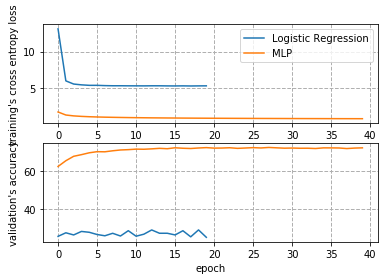
\includegraphics[width=0.45\textwidth]{images/bitmaps_mlp.png}
\caption{Results for a Logistic Regression and a MLP}
\label{fig:mlp_logistic}
\end{figure}

Without much surprise, a model as simple as the logistic regression performs poorly on this classification task. However, the simple MLP already achieves a fairly good accuracy for this kind of task. Indeed there is a fair amount of classes and the data intuitively doesn't seem easy to exploit because drawings are more abstract than pictures and their quality can be quite different from one drawing to another (see \ref{fig:bitmap_drums}). Besides 28x28 bitmaps are small and grayscale. This is why we don't expect to obtain the same results as one can achieve on ImageNet.

\subsubsection{ResNet18, ResNet34, and MobileNet from scratch}

Then, we train three tried and proven image classification CNN models from scratch: ResNet18, ResNet34, and MobileNet. These models expect an RGB image as the input (ideally its size should be 224x224). To process grayscale bitmaps, we just adapt the first convolutional layer of the models to take only one channel as their input instead of three. Of course, we also adapt the last fully connected layer of the classifier to have 100 outputs instead of 1000 (there are 1000 classes on ImageNet). Finally, it is possible to use these models with small 28x28 images because they all have an adaptive average pool layer before their classifier. The output of this layer doesn't depend on the input size.

We train them for 20 epochs by using a Stochastic Gradient Descent (SGD) with a learning rate of 0.005 as the optimizer. The loss is measured by using Cross Entropy Loss. Results are shown in figure \ref{fig:cnn_scratch}. The models achieve an accuracy of, respectively, 83.08\%, 83.29\%, and 81.9\% on the validation set. However, while the ResNet models fit the data pretty quickly, the MobileNet model clearly doesn't converge to its minimal generalization loss in less than 20 epochs so this model can most likely perform better if we train it longer.

\begin{figure}[h] 
\centering
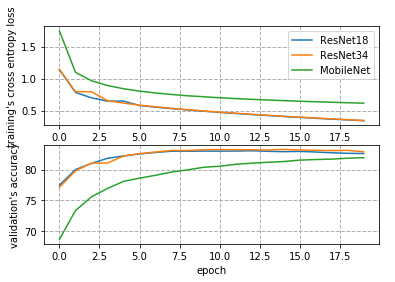
\includegraphics[width=0.45\textwidth]{images/cnn_scratch_results.png}
\caption{Results for popular CNN models trained from scratch}
\label{fig:cnn_scratch}
\end{figure}

\subsubsection{Transfer Learning from ResNet18, ResNet34, and MobileNet}

The idea behind training these models from scratch is that transfer learning doesn't necessarily apply to our problem. Indeed, these models are pre-trained on ImageNet on a different classification task involving large RGB pictures. When trying to do simple transfer learning (only training the last fully connected layer of the model, a.k.a the classifier), we get extremely poor results that are not shown here.

However, it appears pre-trained models still learned useful features for our problem on the ImageNet dataset. Their weights are closer to the minimal generalization loss as we show by fine-tuning the same models, trained in the exact same way, but with their weights initialized to the values learned on the ImageNet dataset.

To use these models, we need to adapt our dataset. We just repeat three times the channel dimension of our 1x28x28 tensors to get 3x28x28 tensors. We then normalize the data by using the mean and standard deviation from ImageNet. Of course, we also adapt the last fully connected layer of the classifier to have 100 outputs instead of 1000.

The results of this approach are shown in figure \ref{fig:cnn_pretrained}. The pre-trained models clearly outperform their \textit{from-sratch}-counterpart, achieving 84.35\%, 84.59\%, and 84.81\% accuracies on the validation set (for ResNet18, ResNet34, and MobileNet respectively).

\begin{figure}[h] 
\centering
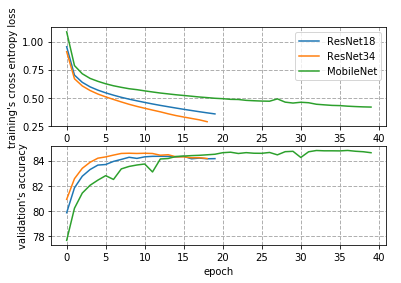
\includegraphics[width=0.45\textwidth]{images/cnn_pretrained_results.png}
\caption{Results for pretrained, fine-tuned CNN models}
\label{fig:cnn_pretrained}
\end{figure}

It should be noted that when the MobileNet model is trained longer (40 epochs here), it outperforms the ResNet18 and ResNet34 models on our problem. We don't train ResNet18 and ResNet34 for 40 epochs because their validation accuracy starts decreasing after only 9 to 13 epochs (and it would take too much time to wait for 40 epochs just to see how much the validation accuracy would decrease).

\subsubsection{ResNet18 with a modified convolution layer}

Finally, we try to adapt the ResNet18 architecture to better fit our problem. Clearly, MobileNet outperforms ResNet18 on this problem. One of the reasons could be the first convolutional layer of the architecture. Indeed, these layers are different:

\begin{itemize}
    \item For ResNet18, it is a layer with 64 output channels, 7x7 kernels, 2x2 stride, and 3x3 padding.
    \item For MobileNet, it is a layer with 32 output channels, 3x3 kernels, 2x2 stride, and 1x1 padding.
\end{itemize}

Having smaller kernels seems to particularly make sense for small 28x28 images. For this reason, we adapt the ResNet18 architecture by replacing its first convolutional layer by a layer with 64 output channels, 3x3 kernels, 2x2 stride, and 1x1 padding. Of course, we cannot use the pre-trained version of ResNet18 after changing the very first layer because the weights in the following layers no longer make any sense (trying to do so leads to very poor results).

This is why we train this new architecture from scratch by using a SGD with a learning rate of 0.02 (we use a higher learning rate for faster convergence). The results are shown in figure \ref{fig:cnn_adapted} with the previous results of ResNet34, which was the best model trained from scratch.

\begin{figure}[h] 
\centering
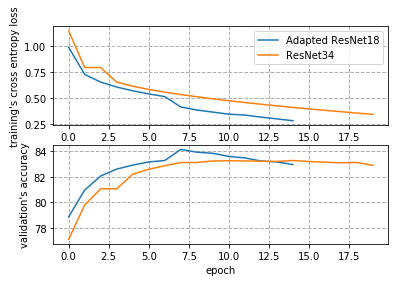
\includegraphics[width=0.45\textwidth]{images/cnn_adapted_results.png}
\caption{Results for the adapted ResNet18 model}
\label{fig:cnn_adapted}
\end{figure}

The adapted ResNet18 achieves an accuracy of 84.15\% on the validation set. This means it outperforms the previous three models that are trained from scratch, which is a pretty good result for such an experiment. It also goes to show that our intuition is likely correct: the small kernels in the MobileNet architecture are more suited to our problem than the bigger ones in the ResNet architecture. It may be possible to further adapt the ResNet architecture to get a model that performs even better.

Unfortunately, it does not outperform the pre-trained MobileNet model. Besides, we are not sure that a MobileNet trained from scratch would not outperform the adapted ResNet18 after more than 20 epochs. We could also try to train a ResNet34 with an adapted first convolutional layer but this would take us too much time.

Note that the adapted ResNet18 converges faster in figure \ref{fig:cnn_adapted} because a higher learning rate is used in the SGD.

\subsubsection{Global Comparison}

To conclude, we show the results of every model for the 28x28 grayscale bitmaps approach in table \ref{tab:cnn_every_results}. The model that performs best on our problem is the pre-trained, fine-tuned MobileNet.

\begin{table}[h]
    \centering
    \begin{tabular}{c|c}
    \textbf{Model}                      & \textbf{Validation accuracy} \\
    Logistic Regression                 & 28.84\%             \\
    MLP (from scratch)                  & 72.69\%             \\
    ResNet18 (from scratch)             & 83.08\%             \\
    ResNet34 (from scratch)             & 83.29\%             \\
    MobileNet (from scratch)            & 81.9\%              \\
    Adapted ResNet18 (from scratch)     & 84.15\%             \\
    ResNet18 (pre-trained, fine-tuned)  & 84.35\%             \\
    ResNet34 (pre-trained, fine-tuned)  & 84.59\%             \\
    MobileNet (pre-trained, fine-tuned) & 84.81\%            
    \end{tabular}
    \caption{Results for every model}
    \label{tab:cnn_every_results}
\end{table}

%------------------------------------------------------------------------
\subsection{\imgenTitle{}}
In this section we mostly use the same models as for the previous one with richer dataset to try and boost the validation accuracy.
We can see that we consistently achieve better results using pretrained models so we choose to only use those. We focus on resnet18 and mobilenet.

First we want to know if an increased resolution can boost the results. For this purpose, we use the drawing strokes to render 3x64x64 and 3x64x64 tensors and normalize the data using the mean and standard deviation from the pretrained model. The results of the resnet18 model for this approach are shown in figure \ref{fig:resnet_64_3k}.


\begin{figure}[h] 
\centering
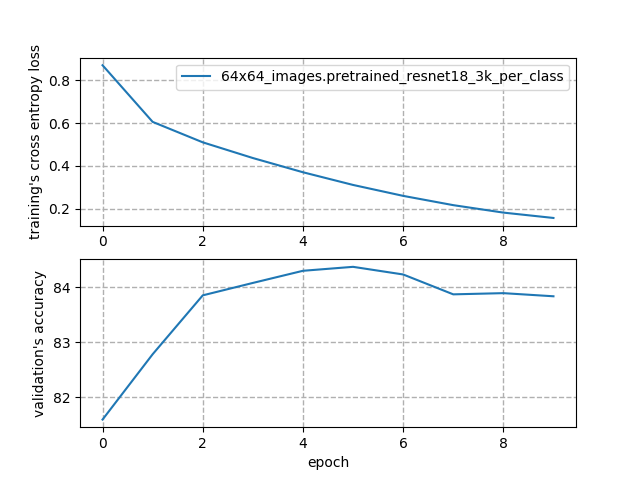
\includegraphics[width=0.45\textwidth]{images/imgen_resnet18_3k.png}
\caption{Results for the pretrained ResNet18 model on 64x64 images}
\label{fig:resnet_64_3k}
\end{figure}


We achieve a validation accuracy of 84.37\% which is on par with the same model trained on 28x28 images, though the total number of images was different: 20k vs 3k. These results are promising so we can try the same thing with more images.

\begin{figure}[h] 
\centering
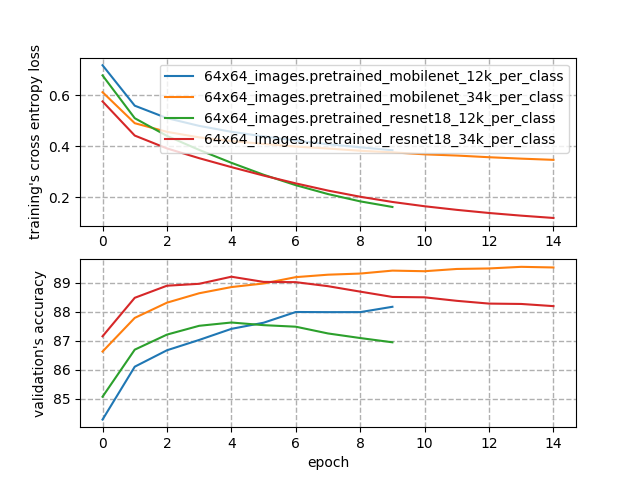
\includegraphics[width=0.45\textwidth]{images/imgen_64.png}
\caption{Results for the pretrained models 64x64 images}
\label{fig:imgen_64}
\end{figure}

This time we achieve a validation accuracy of 88.18\% on mobilenet and 87.64\% on resnet18 on 12k images and 89.55\% and 89.22\% on 34k images, as can be seen on figure \ref{fig:imgen_64}. We see that the results consistently improve as we add more images to train on, so we can safely say that training on 64x64 images yields better results than on the 28x28 ones. Indeed, with 3k images we already have the same results as with 20k previously.

In the end, we try increasing the resolution even further at 96x96, still with 34k images. The results on figure \ref{fig:imgen_96} show an even better validation accuracy of 90.10\% on mobilenet and 89.57\% on resnet18. Thus we can conclude than both the number of images and the resolution of such images is helping the results we can get on a given set of models.

\begin{figure}[h] 
\centering
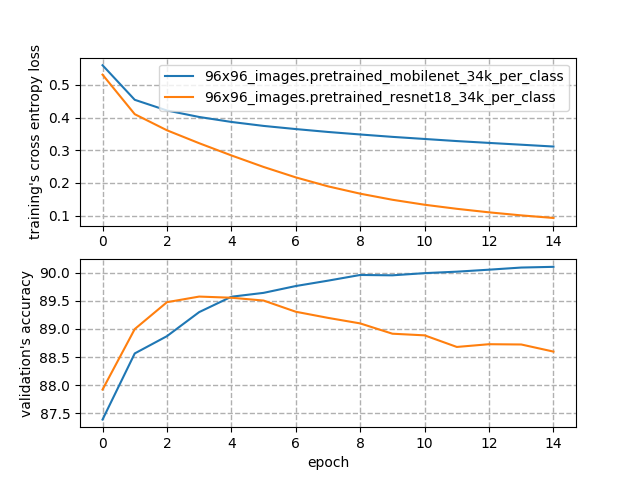
\includegraphics[width=0.45\textwidth]{images/imgen_96.png}
\caption{Results for the pretrained models 96x96 images}
\label{fig:imgen_96}
\end{figure}


%------------------------------------------------------------------------
\subsection{Putting it all together}

In this section we present the results of the best models of each approach on the test dataset (first $20,000$ samples of each class).
The results are displayed on table \ref{tab:final_results}.

\begin{table}[h]
    \centering
    \begin{tabular}{|c|c|c|c|c}
        \hline
          \textbf{Approach} & \textbf{Model Name} & \textbf{Test Accuracy}  \\
          \hline\hline
         RNNs on strokes & BiConvBiLSTM & $87.44\space \%$ \\
          \hline
         \multirow{1}{4em}{CNNs on 28x28 images} & Fine-tuned ResNet34 & $84.62\space \%$ \\
         & Fine-tuned MobileNet & $84.84\space \%$ \\
         & Adapted ResNet34 & $84.12\space \%$ \\
          \hline
         \multirow{4}{4em}{CNNs on generated images} & MobileNet on 64x64 & $91.03\space \%$ \\
         & MobileNet on 96x96 & $92.18\space \%$ \\
         & ResNet18 on 64x64 & $92.18\space \%$ \\
         & ResNet18 on 96x96 & $92.44\space \%$ \\
         \hline
    \end{tabular}
    \caption{Results of the best models on the test dataset}
    \label{tab:final_results}
\end{table}

Of course, these results are not directly comparable as we don't use the same amount of data to train all these models. However, it should be stressed that there is a tradeoff to take into account between performance and training time. In particular, we never use the full dataset for the most complex models because of the time taken to train them, or because of practical issues such as the data size in memory.

Even with a fair comparison though (see previous subsections), we can conclude that the third approach we tried, namely CNNs on generated images, yields the best performance for our classification task.

%------------------------------------------------------------------------
\section{Conclusion}

This project allowed us to have a better understanding of Deep Learning architectures such as RNNs and CNNs and to apply them on a real-world case. Moreover, it greatly improved our knowledge of the PyTorch deep learning framework which we based our study on.

To improve our current results, we already have some leads that would be interesting to explore.

First, we could try to tweak some hyper parameters of our trained models that we did not tinker with such as: learning rates, batch sizes, optimizers. For more specific improvements, for the LSTMs models we could use sliding windows instead of fixed padding / cropping to increase the number of samples available per class and hence be able to train models and more data.

We could try many more CNN models on generated images, for instance DenseNet, VGG, Inception, Se-Resnext.

One idea that, had we had more time, we would have liked to explore is, for CNNs on generated images, the progressive resizing of all images while training the CNN, from smaller to bigger sizes. \cite{ProgressiveResizing} Empirically, this technique allows for better performance on some image recognition tasks.

We could also use multiple models and make them vote as a group such as in an ensemble learning method, this would probably yield better results than using only one model.

Finally, training the best models on more data would surely yield much better performances ($75,000$ training images per class instead of $34,000$ for the ResNet18 on 96x96 generated images), however this would require much more computation capabilities and much more time to train.

{\small
\bibliographystyle{ieee_fullname}
\bibliography{egbib}
}

\end{document}
